\section[Experimente]{Experimente}

\begin{frame}[<+->]
\frametitle{Rolling Stone}
\begin{minipage}[c]{0.39\textwidth}
% \vspace*{-1.5cm}
%   \includegraphics[width=\linewidth]{../dipl_tex/img/tikz/rolling-stones.pdf} \\
%   \includegraphics[width=1.05\linewidth]{../dipl_tex/img/tikz/rolling-stones-solution.pdf}
\scalebox{1.07}{\documentclass{standalone}
\IfStandalone{
	\usepackage{pgfplots,pgfplotstable}
	\usetikzlibrary{external}
	
	}{%
}
% \usepackage{pgfplots,pgfplotstable}
% \usetikzlibrary{external}
	

\begin{document}
\tikzsetnextfilename{rolling-stones}
\begin{tikzpicture}[x=3em,y=3em]
\begin{axis}[
            xmin=-2.5,xmax=2.5,
            ymin=-1.5,ymax=1.5,
            xlabel=$z$,
%             legend entries={$V(z)$,$V'(z)$},
            width=\linewidth
        ]
        \addplot[domain=-2.5:-1]{(1+x)^2/2};
        \addplot[-,domain=-1:1]{0};
        \addplot[domain=1:2.5]{(1-x)^2/2};
        \addplot[domain=-2.5:2.5,samples=100,blue]{-min(max(-1-x,0),1-x)};
\end{axis}
\end{tikzpicture}

 
\end{document}
}
\scalebox{1.2}{\documentclass{standalone}
\IfStandalone{
	\usepackage{pgfplots,pgfplotstable}
	\usetikzlibrary{external}
	
	}{%
}
\begin{document}
\tikzsetnextfilename{rolling-stones-solution}
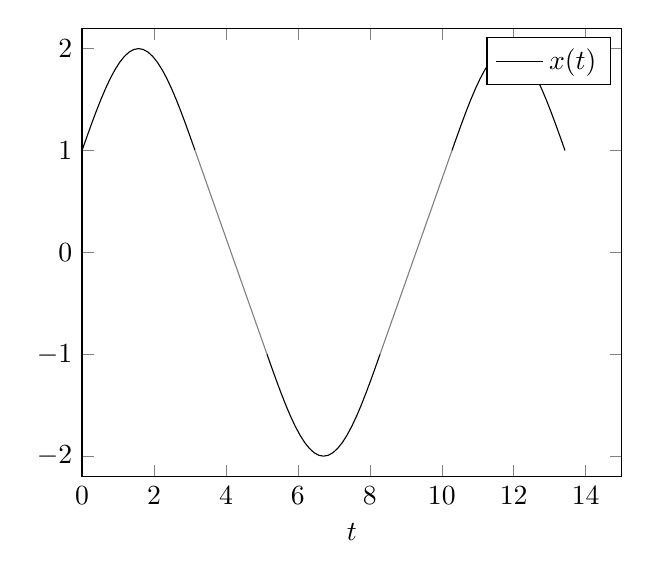
\begin{tikzpicture}[x=3em,y=3em]
\begin{axis}[
            xmin=0,xmax=15,
            ymin=-2.2,ymax=2.2,
            xlabel=$t$,
            legend entries={$x(t)$}
        ]
        \addplot[domain=0:3.14]{1+sin(deg(x))};
        \addplot[domain=pi:pi+2,gray]{1-x+pi};
        \addplot[domain=pi+2:2*pi+2]{-1-sin(deg(2-x))};
        \addplot[domain=2*pi+2:2*pi+4,gray]{x-3-2*pi};
        \addplot[domain=2*pi+4:3*pi+4]{1+sin(deg(x-2*pi-4))};
\end{axis}
\end{tikzpicture} 
\end{document}
}
\end{minipage}
\hfill
\begin{minipage}[c]{0.6\textwidth}
% \vspace*{-0.3cm}
Definiere $\ddot x = -V'(z)$ und 
\[
 V(z) = 
 \begin{cases}
 \frac{(1+z)^2}{2} & z\leq -1\\
 \frac{(1-z)^2}{2} &  z\geq 1\\
  0 & \text{sonst}
 \end{cases},
\]
$ V'(z) = \min(\max(-z-1,0),1-z)$
\pause
\begin{block}{Rolling Stone}
\centering
  $
  \begin{pmatrix}
   \dot x_1 \\
   \dot x_2 \\
  \end{pmatrix}
 = 
 \begin{pmatrix}
  x_2 \\
  -x_1 - \frac{|x_1-1|}{2} + \frac{|x_1+1|}{2}
 \end{pmatrix}
$
\end{block}
% Ist in Abs Normal Form darstellbar:
\vspace*{-0.5cm}
\pause
\[
\begin{aligned}
c = \begin{pmatrix}
     -1\\
     1
    \end{pmatrix}
& 
 Z = \begin{pmatrix}
      1 & 0 \\
      1 & 0
     \end{pmatrix} 
 \\
J = \begin{pmatrix}
      0&1\\
      -1 & 0
     \end{pmatrix}
 &
 Y = \begin{pmatrix}
      0 & 0\\
      -0.5  & 0.5
     \end{pmatrix}
\end{aligned}
\]
\end{minipage}
\end{frame}
\begin{frame}[<+->]
\frametitle{Rolling Stone Adjungierte Gleichung Konvergenz}
\centering
% \includegraphics[width=0.8\linewidth]{../dipl_tex/img/tikz/convergence_rolling_plot.pdf} \\
\documentclass{standalone}
\IfStandalone{
	\usepackage{pgfplots,pgfplotstable}
	\usetikzlibrary{external}
	\newcommand{\fromRoot}[1]{../#1}
}{%
}
\begin{document}
\tikzsetnextfilename{convergence_rolling_plot}
\begin{tikzpicture}
\begin{loglogaxis}[
	width=10cm,
	xlabel=Degrees of freedom $N$,
	ylabel=Error at time $T$,
	legend entries ={Expl. MP,
	IMP,
	GIMP, 
	}
]
  	\addplot[mark=none,red,very thin] table[x index=0,y index=2] {img/data/convergence_rolling_plot.dat};%expl midpoint
 	\addplot[mark=none,green,very thin] table[x index=0,y index=3] {img/data/convergence_rolling_plot.dat};%impl midpoint
	\addplot[mark=none,blue,very thin] table[x index=0,y index=1] {img/data/convergence_rolling_plot.dat};%gen midpoint

	\addplot[mark=none,very thin,gray, yshift=-20pt] 
		table[y={create col/linear regression={x=0,y=1}}] {img/data/convergence_rolling_plot.dat}
		  coordinate [pos=0.5] (A)
		  coordinate [pos=0.6] (B)
		;
	% save the slope parameter:
	\pgfmathparse{-\pgfplotstableregressiona}	
	\pgfmathsetmacro{\slope}{\pgfmathresult}
	
	% draw the opposite and adjacent sides
	% of the triangle
	\draw[very thin,gray] (B) -| (A)
	node [pos=0.2,anchor=north]
	{\pgfmathprintnumber{\slope}};
\end{loglogaxis}
\end{tikzpicture}
\end{document} 
\end{frame}
\begin{frame}[<+->]
\frametitle{Rolling Stone Adjungierte Gleichung}
\begin{minipage}[c]{0.45\textwidth}
\centering
% \includegraphics[width=1.02\linewidth]{../dipl_tex/img/tikz/rolling_jac_da_gradient1_imp.pdf} \\
\documentclass{standalone}
\IfStandalone{
	\usepackage{pgfplots,pgfplotstable}
	\usetikzlibrary{external}
	\newcommand{\fromRoot}[1]{../#1}
}{%
}
\begin{document}
\tikzsetnextfilename{rolling_jac_da_gradient1_imp}
\begin{tikzpicture}
    \begin{axis}[view={-20}{60}, grid=both,width=\linewidth,
%      title={$\sfrac{\partial J}{\partial x_0^{(1)}}$},
    xlabel={$x_0^{(0)}$},
    ylabel={$x_0^{(1)}$},
    zlabel={$\sfrac{\partial J}{\partial x_0^{(1)}}$}]
      \addplot3[surf] file {\fromRoot img/data/grad1_impl.dat};
    \end{axis}
\end{tikzpicture}
\end{document} 
(a) IMP
\end{minipage}
\begin{minipage}[c]{0.45\textwidth}
\centering
% \includegraphics[width=1.02\linewidth]{../dipl_tex/img/tikz/rolling_jac_da_gradient1.pdf} 
\documentclass{standalone}
\usepackage{pgfplots,pgfplotstable}
\IfStandalone{
	\usepackage{pgfplots,pgfplotstable}
	\usetikzlibrary{external}
	\newcommand{\fromRoot}[1]{../#1}
}{%
}
\begin{document}
\tikzsetnextfilename{rolling_jac_da_gradient1}
\begin{tikzpicture}
    \begin{axis}[view={-20}{60}, grid=both,width=\linewidth,
%      title={$\sfrac{\partial J}{\partial x_0^{(1)}}$},
    xlabel={$x_0^{(0)}$},
    ylabel={$x_0^{(1)}$},
    zlabel={$\sfrac{\partial J}{\partial x_0^{(1)}}$}]
      \addplot3[surf] file {img/data/grad1_gimp.dat};
    \end{axis}
\end{tikzpicture}
\end{document}
(b) GIMP
\end{minipage}
\hfill
\centering
\\[0.6cm]
$\xobs$ - Exakte Lösung für $x_0=(1,1)$
\end{frame}

\begin{frame}[<+->]
\frametitle{Rolling Stone Convergence}
\centering
\begin{minipage}[c]{0.49\textwidth}
\centering
\documentclass{standalone}
\IfStandalone{
	\usepackage{pgfplots,pgfplotstable}
	\usetikzlibrary{external}
	\newcommand{\fromRoot}[1]{../#1}
}{%
}
\begin{document}
\tikzsetnextfilename{rolling_convergence_adjoint_discrete}
\begin{tikzpicture}
\begin{loglogaxis}[
	width=\linewidth,
	xlabel=Anzahl der Freiheitsgrade $N$,
	ylabel=Fehler in $x$,
	legend entries ={Expl. MP,
	IMP,
	GIMP, 
	}
]
  	\addplot[mark=none,red,very thin] table[x index=0,y index=3] {img/data/rolling_convergence_adjoint_discrete.dat};%expl midpoint
 	\addplot[mark=none,green,very thin] table[x index=0,y index=2] {img/data/rolling_convergence_adjoint_discrete.dat};%impl midpoint
	\addplot[mark=none,blue,very thin] table[x index=0,y index=1] {img/data/rolling_convergence_adjoint_discrete.dat};%gen midpoint

	\addplot[mark=none,very thin,gray, yshift=-20pt] 
		table[y={create col/linear regression={x=0,y=1}}] {img/data/rolling_convergence_adjoint_discrete.dat}
		  coordinate [pos=0.2] (A)
		  coordinate [pos=0.3] (B)
		;
	% save the slope parameter:
	\pgfmathparse{-\pgfplotstableregressiona}	
	\pgfmathsetmacro{\slope}{\pgfmathresult}
	
	% draw the opposite and adjacent sides
	% of the triangle
	\draw[very thin,gray] (B) -| (A)
	node [pos=0.2,anchor=north]
	{\pgfmathprintnumber{\slope}};
\end{loglogaxis}
\end{tikzpicture}
\end{document} 
% \includegraphics[width=1\linewidth]{../dipl_tex/img/tikz/rolling_convergence_adjoint_discrete.pdf} \\
(a) Diskrete Observierung
\end{minipage}
\hfill
\begin{minipage}[c]{0.49\textwidth}
\centering
% \includegraphics[width=1\linewidth]{../dipl_tex/img/tikz/rolling_convergence_adjoint_smooth.pdf} \\
\documentclass{standalone}
\IfStandalone{
	\usepackage{pgfplots,pgfplotstable}
	\usetikzlibrary{external}
	\newcommand{\fromRoot}[1]{../#1}
}{%
}
\begin{document}
\tikzsetnextfilename{rolling_convergence_adjoint_smooth}
\begin{tikzpicture}
\begin{loglogaxis}[
	width=\linewidth,
	xlabel=Anzahl der Freiheitsgrade $N$,
	ylabel=Fehler in $x$,
	legend entries ={Expl. MP,
	IMP,
	GIMP, 
	}
]
  	\addplot[mark=none,red,very thin] table[x index=0,y index=3] {img/data/rolling_convergence_adjoint_smooth.dat};%expl midpoint
 	\addplot[mark=none,green,very thin] table[x index=0,y index=2] {img/data/rolling_convergence_adjoint_smooth.dat};%impl midpoint
	\addplot[mark=none,blue,very thin] table[x index=0,y index=1] {img/data/rolling_convergence_adjoint_smooth.dat};%gen midpoint

	\addplot[mark=none,very thin,gray, yshift=-20pt] 
		table[y={create col/linear regression={x=0,y=1}}] {img/data/rolling_convergence_adjoint_smooth.dat}
		  coordinate [pos=0.2] (A)
		  coordinate [pos=0.3] (B)
		;
	% save the slope parameter:
	\pgfmathparse{-\pgfplotstableregressiona}	
	\pgfmathsetmacro{\slope}{\pgfmathresult}
	
	% draw the opposite and adjacent sides
	% of the triangle
	\draw[very thin,gray] (B) -| (A)
	node [pos=0.17,anchor=north]
	{\pgfmathprintnumber{\slope}};
\end{loglogaxis}
\end{tikzpicture}
\end{document} 
(b) Glatte Observierung
\end{minipage}

\end{frame}

\begin{frame}[<+->]
\frametitle{Rolling Stone Optimierung}
\begin{minipage}[c]{0.49\textwidth}
\centering
% \includegraphics[width=1.02\linewidth]{../dipl_tex/img/tikz/rolling_opt2_cost.pdf} \\
\documentclass{standalone}
\usepackage{pgfplots,pgfplotstable}
\IfStandalone{
	\usepackage{pgfplots,pgfplotstable}
	\usetikzlibrary{external}
	\newcommand{\fromRoot}[1]{../#1}
}{%
}
\begin{document}
\tikzsetnextfilename{rolling_opt2_cost}
\begin{tikzpicture}
    \begin{axis}[view={0}{90},
    width=\linewidth,
    legend entries ={Kostenfunktional,IMP, GIMP},
    legend style={at={(0.97,1.40)}},
%     legend style={at={(1.00,0.15)},anchor=east}
    xlabel={$x_0^{(0)}$},
    ylabel={$x_0^{(1)}$},
    zlabel={$\sfrac{\partial J}{\partial x_0^{(1)}}$}]
%     \addplot3[surf] file {img/data/rolling_costfunctional.dat};
     \addplot3[contour gnuplot] file {img/data/rolling_costfunctional.dat};
    \addplot3[mark=o, red] table {img/data/rolling_opt2_iterationSteps.dat};
    \addplot3[mark=o, yellow] table {img/data/rolling_opt2_iterationSteps_impl.dat};
        \end{axis}
\end{tikzpicture}
\end{document} 
\end{minipage}
\hfill
\begin{minipage}[c]{0.49\textwidth}
\centering
% \includegraphics[width=1.02\linewidth]{../dipl_tex/img/tikz/rolling_opt2_convergence.pdf} 
\documentclass{standalone}
\usepackage{pgfplots,pgfplotstable}
\IfStandalone{
	\usepackage{pgfplots,pgfplotstable}
	\usetikzlibrary{external}
	\newcommand{\fromRoot}[1]{../#1}
}{%
}
\begin{document}
\tikzsetnextfilename{rolling_opt2_convergence}
\begin{tikzpicture}
\begin{loglogaxis}[
	width=\linewidth,
	xlabel=Optimierungsschritte,
	ylabel=Fehler,
% 	title=Convergence of Optimization for Rolling Stones,
	legend entries ={IMP,GIMP},
	legend style={at={(0.5,1.0)},anchor=south},
	legend columns=2
]
 	\addplot[mark=none,green,very thin] table[x index=0,y index=2] {img/data/rolling_opt2_convergence.dat};%impl midpoint
	\addplot[mark=none,blue,very thin] table[x index=0,y index=1] {img/data/rolling_opt2_convergence.dat};%gen midpoint
 \end{loglogaxis}
\end{tikzpicture}

\end{document}  
\end{minipage}
\centering
$
x_0^{(\text{Start})}=(0,-1.45) 
$

\end{frame}


\begin{frame}[<+->]
\frametitle{LC Diode}
\begin{block}{LC Diode}
\vspace*{-0.3cm}
\[
 \begin{pmatrix}
  \dot x_1\\
  \dot x_2\\
  \dot x_3\\
 \end{pmatrix}
 = 
 \begin{pmatrix}
  1\\
  x_3\\
  -\left(x_2-CV(x_1) + g(Cx_3)\right)\frac{1}{LC}
 \end{pmatrix},
 g(z) = \begin{cases}
      \alpha z & z> 0,\\
      \beta z & z< 0,\\
0 & \text{sonst}
      \end{cases}
\]
\end{block}
\begin{minipage}{0.45\linewidth}
\documentclass{standalone}
\usepackage{pgfplots,pgfplotstable,circuitikz}

\usetikzlibrary{external}

\begin{document}

\tikzsetnextfilename{lc-circuit}
\begin{tikzpicture}[x=1.5cm]
% \draw[help lines] (0,0) grid (5,3);
% \draw (0,0) 
%     to[L] (0,3) 
%     to (2,3) 
%     to[C=$C$] (3,3)
%     to (5,3)
%     to[diode] (5,0) 
%     to (0,0);
%     to[V,v=$U_q$] (0,2) % The voltage source
\draw (0,0) 
    to (3,0)
    to[V,v=$V(t)$] (3,1.5) % The voltage source
    to[diode] (3,3) 
    to (3,3)
    to[C=$C$] (0,3)
%     to (0,3)
    to[L=$L$](0,0) 
    to (0,0);
    % \draw (2,0) to[C] (2,3);
% \draw (3,0) to[C] (3,3);
% \draw (2.5,0) node[ground] {};
\draw (2.7,2.7) node[anchor=north east,align=right] {$g(x)$};
\draw (2.1,0) node[anchor=north east,align=right] {$I(t)=z(t)$};
% \draw (1.8,1.5) node[anchor=north east] {$C_1$};
% \draw (2.8,1.5) node[anchor=north east] {$C_2$};
% \draw (-0.2,1.5) node[anchor=north east] {$L$};
\end{tikzpicture}

 
\end{document}

\end{minipage}
\begin{minipage}{0.45\linewidth}
\centering
\begin{itemize}
\item $x_1$ Zeit
 \item $x_2$~Ladung~des~Kondensators
 \item $x_3$ Elektrische Stromstärke
\end{itemize}
 $\begin{aligned}
L= 10^{-6}, C=10^{-13}, \omega=3\cdot 10^{9},\\
\alpha =0.5,\beta=10^{5}, V(t) = \sin(\omega t)   
  \end{aligned}
$
 \pause
\begin{align*}
 \Rightarrow g(z) &= \alpha\frac{z+|z|}{2} + \beta\frac{z-|z|}{2}
 \end{align*}
\end{minipage}
 \end{frame}
 \begin{frame}[<+->]
\frametitle{LC Diode Lösung}
\begin{minipage}{0.45\linewidth}
\documentclass{standalone}
\usepackage{pgfplots,pgfplotstable}
\IfStandalone{
	\usepackage{pgfplots,pgfplotstable}
	\usetikzlibrary{external}
	\newcommand{\fromRoot}[1]{../#1}
}{%
}
\begin{document}
\tikzsetnextfilename{lc_solution}
\begin{tikzpicture}
\begin{axis}[
	width=\linewidth,
	legend entries ={$Q(t)$},
	xmin=-1E-12,
	xmax=1.5E-8,
	ymin=-1E-16,
 	ymax=2E-13,
 	xlabel=$x_1$,
 	ylabel=$x_2$
]
	%\addplot[mark=none,blue,dashed] table[x=t,y=x]{grad.dat};
% 	\addplot[mark=none,red,very thin] table[x=t,y=x]{j.dat};
% 	 \addplot[blue,very thin] table[x index=0,y index=2] {dat/sol.dat};
 \addplot[blue] table[x index=0,y index=2] {\fromRoot img/data/lc_solution.dat};
\end{axis}
\end{tikzpicture}
\end{document}  
\end{minipage}  
\begin{minipage}{0.45\linewidth}
\documentclass{standalone}
\usepackage{pgfplots,pgfplotstable}
\IfStandalone{
	\usepackage{pgfplots,pgfplotstable}
	\usetikzlibrary{external}
	\newcommand{\fromRoot}[1]{../#1}
}{%
}
\begin{document}
\tikzsetnextfilename{lc_solution2}

\begin{tikzpicture}
\begin{axis}[
	width=\linewidth,
	legend entries ={$I(t)$},
	xmin=-1E-12,
	xmax=1.5E-8,
	ymin=-5E-5,
 	ymax=3E-4,
 	xlabel=$x_1$,
 	ylabel=$x_3$
]
	%\addplot[mark=none,blue,dashed] table[x=t,y=x]{grad.dat};
% 	\addplot[mark=none,red,very thin] table[x=t,y=x]{j.dat};
	 \addplot[red,very thin] table[x index=0,y index=3] {\fromRoot img/data/lc_solution.dat};

\end{axis}
\end{tikzpicture}
\end{document}  
\end{minipage}
\centering
\\[0.3cm]
Lösung der LC Diode für $x_0=(0,0,0)$
\end{frame}

\begin{frame}[<+->]
\frametitle{LC Diode Konvergenz}
\centering
\scalebox{0.9}{\documentclass{standalone}
\IfStandalone{
	\usepackage{pgfplots,pgfplotstable}
	\usetikzlibrary{external}
	\newcommand{\fromRoot}[1]{../#1}
}{%
}
\begin{document}
\tikzsetnextfilename{lc_convergence}
\begin{tikzpicture}
\begin{loglogaxis}[
% 	width=10cm,
	width=\linewidth,
	xlabel=Anzahl der Freiheitsgrade $N$,
% 	ylabel=Fehler in zum Zeitpunkt $T$,
	ymin=1E-13,
 	ymax=4E-7,
	legend entries ={Expl. MP,
	IMP,
	GIMP, 
	},
	legend style={at={(0.5,1.0)},anchor=south},
	legend columns=3
]
  	\addplot[mark=none,red,very thin] table[x index=0,y index=3] {\fromRoot img/data/lc_convergence.dat};%expl midpoint
 	\addplot[mark=none,green,very thin] table[x index=0,y index=2] {\fromRoot img/data/lc_convergence.dat};%impl midpoint
	\addplot[mark=none,blue,very thin] table[x index=0,y index=1] {\fromRoot img/data/lc_convergence.dat};%gen midpoint

	\addplot[mark=none,very thin,gray, yshift=-20pt] 
		table[y={create col/linear regression={x=0,y=1}}] {\fromRoot img/data/lc_convergence.dat}
		  coordinate [pos=0.5] (A)
		  coordinate [pos=0.6] (B)
		;
	% save the slope parameter:
	\pgfmathparse{-\pgfplotstableregressiona}	
	\pgfmathsetmacro{\slope}{\pgfmathresult}
	
	% draw the opposite and adjacent sides
	% of the triangle
	\draw[very thin,gray] (B) -| (A)
	node [pos=0.2,anchor=north]
	{\pgfmathprintnumber{\slope}};
\end{loglogaxis}
\end{tikzpicture}
\end{document} }
\end{frame}

\begin{frame}[<+->]
\frametitle{LC Diode Datenassimilation}
\centering
\begin{block}{Erweiterte LC Diode} 
\[
 \begin{pmatrix}
  \dot x_1\\
  \dot x_2\\
  \dot x_3\\
  \dot \alpha\\
  \dot \beta
 \end{pmatrix}
 = 
 \begin{pmatrix}
  1\\
  x_3\\
  -\left(x_2-CV(x_1) + g(Cx_3)\right)\frac{1}{LC}\\
  0\\
  0
 \end{pmatrix}
\]
\end{block}
\begin{block}{Adjungierte Gleichung}
\centering
  $\dot{ \bar{x}}(t) =  -\frac{\partial F(x(t))}{\partial x}^\tr \bar x(t) +C_{\text{Pr}}^\tr(C_{\text{Pr}}x(t) - x_{\text{obs}}(t)), ~ \bar x(T) =0$
\end{block}

\begin{itemize}
 \item Observierungen \underline{NUR} über $x_1,x_2,x_3$
 \item Optimierung \underline{NUR} über $\alpha$ und $\beta$
 \item \vspace*{-0.45cm} Nutzung der Projektionsmatrix $C_{\text{Pr}}=
 \begin{pmatrix}
  1 &0 &0 &0 &0  \\
  0 &1 &0 &0 &0  \\
  0 &0 &1 &0 &0  \\
 \end{pmatrix}
$
\end{itemize}
\end{frame}

\begin{frame}[<+->]
\frametitle{LC Diode Adjungierte Gleichung Konvergenz}
\begin{minipage}{0.45\linewidth}
\centering
 \documentclass{standalone}
\IfStandalone{
	\usepackage{pgfplots,pgfplotstable}
	\usetikzlibrary{external}
	\newcommand{\fromRoot}[1]{../#1}
}{%
}
\begin{document}
\tikzsetnextfilename{lc_convergence_adjoint_discrete}
\begin{tikzpicture}
\begin{loglogaxis}[
	width=\linewidth,
	xlabel=Anzahl der Freiheitsgrade $N$,
	ylabel=Fehler zu $\nabla J$,
	legend entries ={Expl. MP,
	IMP,
	GIMP 
	},
	ymax=3E-5,
	legend style={at={(0.5,1.0)},anchor=south},
	legend columns=2,
]
	\addplot[mark=none,red,very thin] table[x index=0,y index=3] {\fromRoot img/data/lc_convergence_adjoint_discrete.dat};%expl midpoint
 	\addplot[mark=none,green,very thin] table[x index=0,y index=2] {\fromRoot img/data/lc_convergence_adjoint_discrete.dat};%impl midpoint
	\addplot[mark=none,blue,very thin] table[x index=0,y index=1] {\fromRoot img/data/lc_convergence_adjoint_discrete.dat};%gen midpoint

	\addplot[mark=none,very thin,gray, yshift=-20pt] 
		table[y={create col/linear regression={x=0,y=1}}] {\fromRoot img/data/lc_convergence_adjoint_discrete.dat}
		  coordinate [pos=0.2] (A)
		  coordinate [pos=0.3] (B)
		;
	% save the slope parameter:
	\pgfmathparse{-\pgfplotstableregressiona}	
	\pgfmathsetmacro{\slope}{\pgfmathresult}
	
	% draw the opposite and adjacent sides
	% of the triangle
	\draw[very thin,gray] (B) -| (A)
	node [pos=0.2,anchor=north]
	{\pgfmathprintnumber{\slope}};
\end{loglogaxis}
\end{tikzpicture}
\end{document}
 (a) Diskrete Observierung
\end{minipage}
\begin{minipage}{0.45\linewidth}
\centering
 \documentclass{standalone}
\IfStandalone{
	\usepackage{pgfplots,pgfplotstable}
	\usetikzlibrary{external}
	\newcommand{\fromRoot}[1]{../#1}
}{%
}
\begin{document}
\tikzsetnextfilename{lc_convergence_adjoint_smooth}
\begin{tikzpicture}
\begin{loglogaxis}[
	width=\linewidth,
	xlabel=Anzahl der Freiheitsgrade $N$,
	ylabel=Fehler zu $\nabla J$,
	legend entries ={Expl. MP,
	IMP,
	GIMP 
	},
	ymax=3E-5,
	legend style={at={(0.5,1.0)},anchor=south},
	legend columns=2
]
  	\addplot[mark=none,red,very thin] table[x index=0,y index=3] {\fromRoot img/data/lc_convergence_adjoint_smooth.dat};%expl midpoint
 	\addplot[mark=none,green,very thin] table[x index=0,y index=2] {\fromRoot img/data/lc_convergence_adjoint_smooth.dat};%impl midpoint
	\addplot[mark=none,blue,very thin] table[x index=0,y index=1] {\fromRoot img/data/lc_convergence_adjoint_smooth.dat};%gen midpoint

	\addplot[mark=none,very thin,gray, yshift=-20pt] 
		table[y={create col/linear regression={x=0,y=1}}] {\fromRoot img/data/lc_convergence_adjoint_smooth.dat}
		  coordinate [pos=0.2] (A)
		  coordinate [pos=0.3] (B)
		;
	% save the slope parameter:
	\pgfmathparse{-\pgfplotstableregressiona}	
	\pgfmathsetmacro{\slope}{\pgfmathresult}
	
	% draw the opposite and adjacent sides
	% of the triangle
	\draw[very thin,gray] (B) -| (A)
	node [pos=0.2,anchor=north]
	{\pgfmathprintnumber{\slope}};
\end{loglogaxis}
\end{tikzpicture}
\end{document}
(b) Glatte Observierung
 \end{minipage}
 \centering
 \\[0.3cm]
  $I=[0,10^{-8}],x_0=(0,0,0,10^3,10^{4}),\xobs(0)=(0,0,0,10^4,10^5)$
\end{frame}


\begin{frame}[<+->]
\frametitle{LC Diode Optimierung}
\begin{minipage}{0.45\linewidth}
\centering
 \documentclass{standalone}
\usepackage{pgfplots,pgfplotstable}
\IfStandalone{
	\usepackage{pgfplots,pgfplotstable}
	\usetikzlibrary{external}
	\newcommand{\fromRoot}[1]{../#1}
}{%
}
\begin{document}
\tikzsetnextfilename{lc_opt1_convergence}
\begin{tikzpicture}
\begin{axis}[
	width=\linewidth,
	xlabel=Optimierungsschritte,
	ylabel=Fehler,
% 	title=Convergence of Optimization for Rolling Stones,
	legend entries ={IMP,GIMP},
	legend style={at={(0.5,1.0)},anchor=south},
	legend columns=2
]
  	
 	\addplot[mark=none,green,very thin] table[x index=0,y index=2] {\fromRoot img/data/lc_convergence_opt_new.dat};%impl midpoint
	\addplot[mark=none,blue,very thin] table[x index=0,y index=1] {\fromRoot img/data/lc_convergence_opt_new.dat};%gen midpoint
\end{axis}
\end{tikzpicture}

\end{document}
(a) Abstand zu exakten $\alpha,\beta$
\end{minipage}
\begin{minipage}{0.45\linewidth}
\centering
 \documentclass{standalone}
\usepackage{pgfplots,pgfplotstable}
\IfStandalone{
	\usepackage{pgfplots,pgfplotstable}
	\usetikzlibrary{external}
	\newcommand{\fromRoot}[1]{../#1}
}{%
}
\begin{document}
\tikzsetnextfilename{lc_opt2_convergence}
\begin{tikzpicture}
\begin{loglogaxis}[
	width=\linewidth,
	xlabel=Optimierungsschritte,
	ylabel=Fehler,
% 	title=Convergence of Optimization for Rolling Stones,
	legend entries ={IMP,GIMP},
	legend style={at={(0.5,1.0)},anchor=south},
	legend columns=2
]
  	
 	\addplot[mark=none,green,very thin] table[x index=0,y index=2] {\fromRoot img/data/lc_opt2_convergence.dat};%impl midpoint
	\addplot[mark=none,blue,very thin] table[x index=0,y index=1] {\fromRoot img/data/lc_opt2_convergence.dat};%gen midpoint
\end{loglogaxis}
\end{tikzpicture}

\end{document}
(b) Kostenfunktional
\end{minipage}
 \centering
 \\[0.3cm]
  $N=500,I=[0,10^{-8}],x_0=(0,0,0,10^3,10^{4}),\xobs(0)=(0,0,0,10^4,10^5)$
\end{frame}


\begin{frame}[<+->]
\frametitle{Shallow Water Equation (SWE)}
\begin{minipage}{0.45\linewidth}
\documentclass{standalone}
\usepackage{pgfplots,pgfplotstable}
\IfStandalone{
	\usepackage{pgfplots,pgfplotstable}
	\usetikzlibrary{external}
	\newcommand{\fromRoot}[1]{../#1}
}{%
}
\begin{document}
\tikzsetnextfilename{swe_plot}
\begin{tikzpicture}
\begin{axis}[
   view={-20}{60}, 
   grid=both,
   width=12cm,
    xlabel={Zeit $t$},
    ylabel={Gitter $x$},
    zlabel={$h$},
    ]
\addplot3[surf] file {img/data/swe_plot.dat};
% \addplot3[surf] file {img/data/grad1_gimp.dat};

\end{axis}
\end{tikzpicture}
\end{document}
\end{minipage}
\begin{minipage}{0.54\linewidth}
 \begin{block}{1D Saint Venan System}
     \centering
     $\begin{cases}
 h_t + (hu)_x = 0,\\
 (hu)_t + \left[\frac{(hu)^2}{h} + \frac{g}{2}h^2\right]_x = 0
\end{cases} $
    \end{block}
   \begin{itemize}
    \item Diskretisierung nach Kurganov (\cite{kurganov2007second})
    \item Unglätten durch Flux - Limiter und Eigenwertberechnung
   \end{itemize}                           
\end{minipage}
\pause
\begin{align*}
\minmod(z_1,z_2,\ldots) &= \begin{cases}
                                  \min_j z_j & \text{falls }z_j>0~\forall j\\
                                  \max_j z_j & \text{falls }z_j<0~\forall j\\
                                  0 & \text{sonst}
                                 \end{cases}\\
&= \min(\max(z_1,z_2,z_3),0) + \max(\min(z_1,z_2,z_3),0)                                 
\end{align*}
\end{frame}
% 
% \begin{frame}[<+->]
% \frametitle{SWE Konvergenz}
% \centering
% \begin{minipage}[b]{0.49\linewidth}
% \centering
% \documentclass{standalone}
\IfStandalone{
	\usepackage{pgfplots,pgfplotstable}
	\usetikzlibrary{external}
	\newcommand{\fromRoot}[1]{../#1}
}{%
}
\begin{document}
\tikzsetnextfilename{swe_initial_values}
\begin{tikzpicture}
\begin{axis}[
	width=\linewidth,
% 	grid=both,
	xlabel=$x$,
	ylabel=$h$,
	legend entries ={
	$U_0^{(1)}$,
	$U_0^{(2)}$,
% 	$U_0^{(3)}$,
% 	$U_0^{(4)}$
	},
	legend style={at={(0.5,1.0)},anchor=south},
	legend columns=2
]
      
%       \addplot[mark=none,green,very thin] table[x index=0,y index=2] {\fromRoot img/data/swe_initial_values.dat};%expl midpoint
      \addplot[mark=none,red,very thin] table[x index=0,y index=3] {\fromRoot img/data/swe_initial_values.dat};%expl midpoint
      \addplot[mark=none,blue,very thin] table[x index=0,y index=1] {\fromRoot img/data/swe_initial_values.dat};%expl midpoint
      %       \addplot[mark=none,cyan,very thin] table[x index=0,y index=4] {\fromRoot img/data/swe_initial_values.dat};%expl midpoint
 	\end{axis}
 	%f
\end{tikzpicture}
\end{document}
% (a) $h_0 \sim n\cdot\mathcal N(\mu,L) + 1$
% \end{minipage}
% \begin{minipage}[b]{0.49\linewidth}
% \centering
% \documentclass{standalone}
\IfStandalone{
	\usepackage{pgfplots,pgfplotstable}
	\usetikzlibrary{external}
	\newcommand{\fromRoot}[1]{../#1}
}{%
}
\begin{document}
\tikzsetnextfilename{swe_initial_values_hu}
\begin{tikzpicture}
\begin{axis}[
	width=\linewidth,
% 	grid=both,
	xlabel=$x$,
	ylabel=$hu$,
	legend entries ={
	$U_0^{(1)}$,
	$U_0^{(2)}$,
% 	$x_0^{(3)}$,
% 	$x_0^{(4)}$
	},
	legend style={at={(0.5,1.0)},anchor=south},
	legend columns=2
]
   
%       \addplot[mark=none,green,very thin] table[x index=0,y index=6] {\fromRoot img/data/swe_initial_values.dat};%expl midpoint
      \addplot[mark=none,red,very thin] table[x index=0,y index=7] {\fromRoot img/data/swe_initial_values.dat};%expl midpoint
%       \addplot[mark=none,cyan,very thin] table[x index=0,y index=8] {\fromRoot img/data/swe_initial_values.dat};%expl midpoint
    \addplot[mark=none,blue,very thin] table[x index=0,y index=5] {\fromRoot img/data/swe_initial_values.dat};%expl midpoint
 \end{axis}
 	%tfewfe
\end{tikzpicture}
\end{document}
% (b)  $(hu)_0\sim n\cdot\mathcal N(\mu,L)$
% \end{minipage}
% 
% \end{frame}


\begin{frame}[<+->]
\frametitle{SWE Konvergenz}
\centering
\scalebox{0.9}{\documentclass{standalone}
\IfStandalone{
	\usepackage{pgfplots,pgfplotstable}
	\usetikzlibrary{external}
	\newcommand{\fromRoot}[1]{../#1}
}{%
}
\begin{document}
\tikzsetnextfilename{swe_convergence}
\begin{tikzpicture}
\begin{loglogaxis}[
	width=\linewidth,
% 	grid=both,
	xlabel=Anzahl der Freiheitsgrade $N$,
	ylabel=Fehler in zum Zeitpunkt $T$,
% 	ymin=1E-13,
%  	ymax=4E-7,
	legend entries ={
	Expl. MP,
	IMP,
	GIMP, 
% 	Rom. GIMP,
% 	Rom. IMP
	},
% 	legend style={at={(0.5,1.0)},anchor=south},
% 	legend columns=2
]
  	\addplot[mark=none,red,very thin] table[x index=0,y index=2] {\fromRoot img/data/swe_convergence.dat};%expl midpoint
 	\addplot[mark=none,green,very thin] table[x index=0,y index=3] {\fromRoot img/data/swe_convergence.dat};%impl midpoint
	\addplot[mark=none,blue,very thin] table[x index=0,y index=1] {\fromRoot img/data/swe_convergence.dat};%gen midpoint
% 	\addplot[mark=none,lime,very thin] table[x index=0,y index=5] {\fromRoot img/data/swe_convergence.dat};%gen midpoint impl
% 	\addplot[mark=none,cyan,very thin] table[x index=0,y index=4] {\fromRoot img/data/swe_convergence.dat};%gen midpoint rom
	\addplot[mark=none,very thin,gray, yshift=-20pt] 
		table[y={create col/linear regression={x=0,y=1}}] {\fromRoot img/data/swe_convergence.dat}
		  coordinate [pos=0.5] (A)
		  coordinate [pos=0.6] (B)
		;
	% save the slope parameter:
	\pgfmathparse{-\pgfplotstableregressiona}	
	\pgfmathsetmacro{\slope}{\pgfmathresult}
	
	% draw the opposite and adjacent sides
	% of the triangle
	\draw[very thin,gray] (B) -| (A)
	node [pos=0.2,anchor=north]
	{\pgfmathprintnumber{\slope}};
\end{loglogaxis}
\end{tikzpicture}
\end{document}}
\end{frame}

% \begin{frame}[<+->]
% \frametitle{SWE Adjungierte Gleichung}
% \centering
% \begin{minipage}[b]{0.49\linewidth}
% % \begin{minipage}[t][3cm][t]{5cm}
% \centering
% \documentclass{standalone}
\IfStandalone{
	\usepackage{pgfplots,pgfplotstable}
	\usetikzlibrary{external}
	\newcommand{\fromRoot}[1]{../#1}
}{%
}

\begin{document}
\tikzsetnextfilename{swe_adjoint_eq_2}
\begin{tikzpicture}
\begin{axis}[
	width=\linewidth,
	xlabel=Zeit $t$,
	ylabel=$\dot{\overline{h}}$,
	legend entries ={
	$\dot{\overline{h}}$
	},
% 	legend style={at={(0.5,1.0)},anchor=south},
% 	legend columns=2
]
\foreach \ind in {1,2,...,11}{
  	\addplot[mark=none,blue,very thin] table[x index=0,y index=\ind] {\fromRoot img/data/swe_adjoint_eq_2.dat};%expl midpoint
 }
\end{axis}
\end{tikzpicture}
\end{document}
% (a) $\dot{\overline{h}}$
% \end{minipage}
% %  \quad 
% \begin{minipage}[b]{0.49\linewidth}
% % \begin{minipage}[t][3cm][t]{5cm}
% \centering
% \documentclass{standalone}
\IfStandalone{
	\usepackage{pgfplots,pgfplotstable}
	\usetikzlibrary{external}
	\newcommand{\fromRoot}[1]{../#1}
}{%
}

\begin{document}
\tikzsetnextfilename{swe_adjoint_eq1_2}
\begin{tikzpicture}
\begin{axis}[
	width=\linewidth,
	xlabel=Zeit $t$,
	ylabel=$\dot{\overline{hu}}$,
	legend entries ={
	$\dot{\overline{hu}}$
	},
% 	legend style={at={(0.5,1.0)},anchor=south},
% 	legend columns=2
]
\foreach \ind in {1,2,...,11}{
  	\addplot[mark=none,red,very thin] table[x index=0,y index=\ind] {\fromRoot img/data/swe_adjoint_eq1_2.dat};%expl midpoint
 }
\end{axis}
\end{tikzpicture}
\end{document}
% (b) $\dot{\overline{hu}}$
% \end{minipage}
% \centering
% $I=[0,10], L=100,\Delta x=10,h = 0.05$ und $U_0^{(1)},n=10,\theta=2,\xobs(0)=U_0^{(1)},n_{\text{obs}}=20,\mu_{\text{obs}}=30$
% \end{frame}

\begin{frame}[<+->]
\frametitle{SWE Konvergenz Adjungierte Gleichung}
\begin{minipage}[b]{0.49\linewidth}
% \begin{minipage}[t][3cm][t]{5cm}
\centering
\documentclass{standalone}
\IfStandalone{
	\usepackage{pgfplots,pgfplotstable}
	\usetikzlibrary{external}
	\newcommand{\fromRoot}[1]{../#1}
}{%
}
\begin{document}
\tikzsetnextfilename{swe_convergence_adjoint_discrete_theta_1}
\begin{tikzpicture}
\begin{loglogaxis}[
	width=\linewidth,
	xlabel=Anzahl der Freiheitsgrade $N$,
	ylabel=Fehler zu $\nabla J$,
	legend entries ={Expl. MP,
	IMP,
	GIMP 
	},
% 	ymax=3E-5,
	legend style={at={(0.5,1.0)},anchor=south},
	legend columns=2
]
	\addplot[mark=none,red,very thin] table[x index=0,y index=2] {\fromRoot img_appendix/data/swe_convergence_adjoint_discrete_theta1.dat};%expl midpoint
 	\addplot[mark=none,green,very thin] table[x index=0,y index=3] {\fromRoot img_appendix/data/swe_convergence_adjoint_discrete_theta1.dat};%impl midpoint
	\addplot[mark=none,blue,very thin] table[x index=0,y index=1] {\fromRoot img_appendix/data/swe_convergence_adjoint_discrete_theta1.dat};%gen midpoint

	\addplot[mark=none,very thin,gray, yshift=-20pt] 
		table[y={create col/linear regression={x=t,y=a}}] {\fromRoot img_appendix/data/swe_convergence_adjoint_discrete_theta1.dat}
		  coordinate [pos=0.2] (A)
		  coordinate [pos=0.3] (B)
		;
	% save the slope parameter:
	\pgfmathparse{-\pgfplotstableregressiona}	
	\pgfmathsetmacro{\slope}{\pgfmathresult}
	
	% draw the opposite and adjacent sides
	% of the triangle
	\draw[very thin,gray] (B) -| (A)
	node [pos=0.2,anchor=north]
	{\pgfmathprintnumber{\slope}};
\end{loglogaxis}
\end{tikzpicture}
\end{document}
(a) Diskrete Observierung
\end{minipage}
%  \quad 
\begin{minipage}[b]{0.49\linewidth}
% \begin{minipage}[t][3cm][t]{5cm}
\centering
\documentclass{standalone}
\IfStandalone{
	\usepackage{pgfplots,pgfplotstable}
	\usetikzlibrary{external}
	\newcommand{\fromRoot}[1]{../#1}
}{%
}
\begin{document}
\tikzsetnextfilename{swe_convergence_adjoint_smooth_theta_1}
\begin{tikzpicture}
\begin{loglogaxis}[
	width=\linewidth,
	xlabel=Anzahl der Freiheitsgrade $N$,
	ylabel=Fehler zu $\nabla J$,
	legend entries ={Expl. MP,
	IMP,
	GIMP 
	},
% 	ymax=3E-5,
	legend style={at={(0.5,1.0)},anchor=south},
	legend columns=2
]
	\addplot[mark=none,red,very thin] table[x index=0,y index=2] {\fromRoot img_appendix/data/swe_convergence_adjoint_smooth_theta1.dat};%expl midpoint
 	\addplot[mark=none,green,very thin] table[x index=0,y index=3] {\fromRoot img_appendix/data/swe_convergence_adjoint_smooth_theta1.dat};%impl midpoint
	\addplot[mark=none,blue,very thin] table[x index=0,y index=1] {\fromRoot img_appendix/data/swe_convergence_adjoint_smooth_theta1.dat};%gen midpoint

	\addplot[mark=none,very thin,gray, yshift=-20pt] 
		table[y={create col/linear regression={x=t,y=a}}] {\fromRoot img_appendix/data/swe_convergence_adjoint_smooth_theta1.dat}
		  coordinate [pos=0.2] (A)
		  coordinate [pos=0.3] (B)
		;
	% save the slope parameter:
	\pgfmathparse{-\pgfplotstableregressiona}	
	\pgfmathsetmacro{\slope}{\pgfmathresult}
	
	% draw the opposite and adjacent sides
	% of the triangle
	\draw[very thin,gray] (B) -| (A)
	node [pos=0.2,anchor=north]
	{\pgfmathprintnumber{\slope}};
\end{loglogaxis}
\end{tikzpicture}
\end{document}
(b) Glatte Observierung
\end{minipage}
% \caption{SWE Konvergenz von $\nabla J$ mit $I=[0,50],L=50,\Delta x=10$, $x_0=U_0^{(2)},k=0.5$, $x_{\text{obs}} = U_0^{(2)}, k=2$ und $\theta=1$}
\centering
$I=[0,50],L=50,\Delta x=10$, $n=10$, $\xobs(0) = U_0^{(1)}, n_{\text{obs}}=20,\mu_{\text{obs}}=30$ und $\theta=1$
\end{frame}

\begin{frame}[<+->]
\frametitle{SWE Optimierung}
\centering
\begin{minipage}[b]{0.49\linewidth}
 \centering
\documentclass{standalone}
\IfStandalone{
	\usepackage{pgfplots,pgfplotstable}
	\usetikzlibrary{external}
	\newcommand{\fromRoot}[1]{../#1}
}{%
}
\begin{document}
\tikzsetnextfilename{swe_convergence_opt}
\begin{tikzpicture}
\begin{loglogaxis}[
	width=\linewidth,
% 	grid=both,
	xlabel=Optimierungsschritte,
	ylabel=Fehler zur exakten Lösung,
% 	ymin=1E-13,
%  	ymax=4E-7,
	legend entries ={
% 	Expl. MP,
	IMP,
	GIMP 
% 	Rom. GIMP,
% 	Rom. IMP
	},
	legend style={at={(0.5,1.0)},anchor=south},
	legend columns=2,
]
  	\addplot[mark=none,green,very thin] table[x index=0,y index=2] {\fromRoot img/data/swe_convergence_opt.dat};%expl midpoint
%  	\addplot[mark=none,green,very thin] table[x index=0,y index=3] {\fromRoot img/data/swe_convergence.dat};%impl midpoint
	\addplot[mark=none,blue,very thin] table[x index=0,y index=1] {\fromRoot img/data/swe_convergence_opt.dat};%gen midpoint
% 	\addplot[mark=none,lime,very thin] table[x index=0,y index=5] {\fromRoot img/data/swe_convergence.dat};%gen midpoint impl
% 	\addplot[mark=none,cyan,very thin] table[x index=0,y index=4] {\fromRoot img/data/swe_convergence.dat};%gen midpoint rom
% 	\addplot[mark=none,very thin,gray, yshift=-20pt] 
% 		table[y={create col/linear regression={x=0,y=1}}] {\fromRoot img/data/swe_convergence.dat}
% 		  coordinate [pos=0.5] (A)
% 		  coordinate [pos=0.6] (B)
% 		;
% 	% save the slope parameter:
% 	\pgfmathparse{-\pgfplotstableregressiona}	
% 	\pgfmathsetmacro{\slope}{\pgfmathresult}
% 	
% 	% draw the opposite and adjacent sides
% 	% of the triangle
% 	\draw[very thin,gray] (B) -| (A)
% 	node [pos=0.2,anchor=north]
% 	{\pgfmathprintnumber{\slope}};
	%deufe
\end{loglogaxis}
\end{tikzpicture}
\end{document}
(a) Abstand zur optimalen Lösung
\end{minipage}
\begin{minipage}[b]{0.49\linewidth}
 \centering
\documentclass{standalone}
\IfStandalone{
	\usepackage{pgfplots,pgfplotstable}
	\usetikzlibrary{external}
	\newcommand{\fromRoot}[1]{../#1}
}{%
}
\begin{document}
\tikzsetnextfilename{swe_convergence_opt_jac}
\begin{tikzpicture}
\begin{loglogaxis}[
	width=\linewidth,
% 	grid=both,
	xlabel=Optimierungsschritte,
	ylabel=$J(x)$,
% 	ymin=1E-13,
%  	ymax=4E-7,
	legend entries ={
% 	Expl. MP,
	IMP,
	GIMP 
% 	Rom. GIMP,
% 	Rom. IMP
	},
	legend style={at={(0.5,1.0)},anchor=south},
	legend columns=2
]
  	\addplot[mark=none,green,very thin] table[x index=0,y index=2] {\fromRoot img/data/swe_convergence_opt_jac.dat};%expl midpoint
%  	\addplot[mark=none,green,very thin] table[x index=0,y index=3] {\fromRoot img/data/swe_convergence.dat};%impl midpoint
	\addplot[mark=none,blue,very thin] table[x index=0,y index=1] {\fromRoot img/data/swe_convergence_opt_jac.dat};%gen midpoint
% 	\addplot[mark=none,lime,very thin] table[x index=0,y index=5] {\fromRoot img/data/swe_convergence.dat};%gen midpoint impl
% 	\addplot[mark=none,cyan,very thin] table[x index=0,y index=4] {\fromRoot img/data/swe_convergence.dat};%gen midpoint rom
% 	\addplot[mark=none,very thin,gray, yshift=-20pt] 
% 		table[y={create col/linear regression={x=0,y=1}}] {\fromRoot img/data/swe_convergence.dat}
% 		  coordinate [pos=0.5] (A)
% 		  coordinate [pos=0.6] (B)
% 		;
% 	% save the slope parameter:
% 	\pgfmathparse{-\pgfplotstableregressiona}	
% 	\pgfmathsetmacro{\slope}{\pgfmathresult}
% 	
% 	% draw the opposite and adjacent sides
% 	% of the triangle
% 	\draw[very thin,gray] (B) -| (A)
% 	node [pos=0.2,anchor=north]
% 	{\pgfmathprintnumber{\slope}};
	%deufe
\end{loglogaxis}
\end{tikzpicture}
\end{document}
(b) Kostenfunktional
\end{minipage}
% \caption{SWE Konvergenz Optimierung mit Parametern $I=[0,100],L=100,\Delta x=10$, $x_0=U_0^{(2)},k=0.5$, $x_{\text{obs}} = U_0^{(2)}, k=1$ und $\theta=2$}
$I=[0,50],L=50,\Delta x=10$, $x_0=U_0^{(1)},n=10$, $\xobs(0) = U_0^{(1)}, n_{\text{obs}}=20,\mu_{\text{obs}}=30$ und $\theta=2$

\end{frame}
